\documentclass[conference]{IEEEtran}
\IEEEoverridecommandlockouts
\usepackage{cite}
\usepackage{amsmath,amssymb}
\usepackage{booktabs}
\usepackage{graphicx}
\usepackage{url}
\usepackage{array}
\usepackage{balance}

\title{Conditional Hybrid Retrieval under Recall Budgets: An Indexed Cascade Study}

\author{\IEEEauthorblockN{Ali Omar, Abdallah Mestrah, and Abbas Yazbek}
\IEEEauthorblockA{Lebanese University\\
Supervisor: Dr. Ahmad Abboud}}

\begin{document}
\maketitle

\begin{abstract}
Hybrid retrieval can improve document coverage, but running every retriever for every query adds latency. We implemented a Python hybrid baseline inspired by Blended RAG and then evaluated a BM25-first cascade with a compatible indexed BM25 scorer. The cascade uses a frozen Ridge gate to decide whether to return BM25 results or execute Dense MiniLM and SPLADE before reciprocal rank fusion. On all 50 BEIR TREC-COVID queries, the preselected indexed cascade was 1.24$\times$ faster than equally indexed fusion and retained 96.68\% of its Recall@100. On a fixed sample of 256 SQuAD questions, the fastest cascade was 1.59$\times$ faster than indexed fusion and retained 99.22\%. Indexing alone accounted for much of the larger cross-run speedup against the earlier implementation. These results measure retrieval latency and ranking quality within our Python implementation; they do not establish acceleration of the original Elasticsearch/ELSER system, generated-answer quality, or superiority over every standalone retriever.
\end{abstract}

\begin{IEEEkeywords}
hybrid retrieval, reciprocal rank fusion, BM25, conditional computation, retrieval latency
\end{IEEEkeywords}

\section{Introduction}
Retrieval-augmented generation systems depend on a retrieval stage to supply documents to a downstream language model. Hybrid retrieval combines methods with complementary behavior: lexical matching, semantic vector search, and learned sparse expansion. A static hybrid pipeline runs every branch for every query, even when one branch may already retrieve adequate results.

This study asks whether a BM25-first gate can skip neural retrieval for selected queries while retaining a chosen fraction of the full-fusion Recall@100. We first implemented a Python baseline inspired by Blended RAG, then added a postings-based BM25 scorer and a frozen conditional gate. The gate predicts the nonnegative recall gain that fusion may provide over BM25. It returns the BM25 ranking when the prediction is below a calibrated threshold; otherwise, it runs Dense MiniLM and SPLADE and fuses all three rankings.

The work makes a measured systems contribution rather than claiming a new routing principle. We apply the indexed scorer to both cascade and fusion, report standalone retrievers, and distinguish the indexing gain from the additional routing gain. Query-dependent retrieval and eager BM25 scoring have prior work \cite{adaptive,bm25s}. Our results are specific to the evaluated implementation, collections, and timing setup.

\section{Background and Related Work}
\subsection{Hybrid retrieval}
BM25 scores lexical overlap using term frequency, inverse document frequency, and document-length normalization. Dense retrieval encodes queries and documents as continuous vectors and ranks by vector similarity \cite{sbert}. SPLADE produces learned sparse vocabulary weights, allowing neural term expansion with sparse representations \cite{splade}. These methods can retrieve different relevant documents, so a system may combine their rankings.

Blended RAG combines keyword, dense-vector, and learned sparse retrieval in Elasticsearch, using ELSER for learned sparse retrieval \cite{blended}. Our implementation replaces the engine and sparse model with Python BM25, MiniLM, and SPLADE. It also uses reciprocal rank fusion (RRF), which sums rank-based contributions rather than raw scores:
\begin{equation}
  \operatorname{RRF}(d)=\sum_{m\in M}\frac{1}{k+\operatorname{rank}_{m}(d)},\quad k=60.
\end{equation}
The fixed constant reduces the influence of small rank differences. RRF avoids direct score-scale comparisons across retrievers.

\subsection{Conditional retrieval}
Adaptive retrieval selects or orders retrieval methods based on query properties. This can save computation, but savings depend on the cost of the first stage and the cost of the decision rule. A slow first-stage search can erase the savings from skipped neural branches. Accordingly, this study examines a frozen gate with an indexed BM25 first stage and compares it with equally indexed static fusion.

Prior work studies query-dependent selection between dense and sparse retrieval \cite{adaptive}. BM25S moves work into index construction to speed lexical scoring \cite{bm25s}. We build on these research directions as an empirical systems evaluation. The gate is intentionally small and uses only query and BM25 signals, while the BM25 postings implementation preserves the scoring behavior used by the earlier baseline. We do not claim that either conditional retrieval or eager sparse scoring originates in this study.

The comparison with equally indexed fusion matters because a comparison only against the earlier implementation would combine two changes. We therefore ask three practical questions: how much time does indexed BM25 save while preserving rankings; how much additional mean latency does conditional routing remove; and do the resulting quality-time points compare favorably with individual retrievers?

\section{Method}
\subsection{Retrievers and static fusion}
The static reference runs Best Fields BM25, Dense MiniLM (\texttt{sentence-transformers/all-MiniLM-L6-v2}), and SPLADE (\texttt{naver/splade-cocondenser-ensembledistil}). BM25 searches title and abstract separately and uses the larger field score. Each retriever returns up to 100 documents. RRF combines the ranked lists and returns the top 100.

\subsection{Ridge gate}
The cascade runs BM25 first and computes 11 query and BM25-result features: query token count, unique token count, top-one and top-two BM25 scores, their gap, mean and standard deviation of top-10 scores, top-one score normalized by query length, maximum and mean query-term IDF, and the standard deviation of query-term IDF. These features describe query length, term specificity, and the BM25 score distribution. They do not use relevance labels or neural rankings at inference.

Table~\ref{tab:features} lists the inputs. IDF is inverse document frequency: terms that occur in fewer corpus documents receive larger values. The top-score gap can indicate that one lexical result stands apart from the next, but a gap alone does not guarantee relevance. Ridge combines these signals rather than relying on a single hand-written confidence rule.

\begin{table*}[t]
\centering
\caption{The 11 query-time features used by the frozen Ridge gate.}
\label{tab:features}
\small
\begin{tabular}{ll}
\toprule
Feature & Meaning\\
\midrule
\texttt{query\_token\_count} & Number of query tokens after project tokenization\\
\texttt{query\_unique\_token\_count} & Number of distinct query tokens\\
\texttt{bm25\_top1}, \texttt{bm25\_top2} & Scores of the first- and second-ranked BM25 documents\\
\texttt{bm25\_gap12} & Difference between the top-one and top-two scores\\
\texttt{bm25\_top10\_mean} & Mean BM25 score among the first ten results\\
\texttt{bm25\_top10\_std} & Standard deviation of scores among the first ten results\\
\texttt{bm25\_top1\_per\_query\_token} & Top-one score divided by query token count\\
\texttt{max\_idf}, \texttt{mean\_idf} & Maximum and mean IDF among distinct query terms\\
\texttt{idf\_std} & Standard deviation of IDF across distinct query terms\\
\bottomrule
\end{tabular}
\end{table*}

The training target for query $q$ is the positive recall gain of static fusion over BM25:
\begin{equation}
  y_q=\max\left(R_{\mathrm{fusion},q}@100-R_{\mathrm{BM25},q}@100,0\right).
\end{equation}
A standardized Ridge regression model with $\alpha=10$ predicts this gain. Negative predictions are clipped to zero. The gate compares the prediction $\hat y_q$ with a threshold $\tau$:
\begin{equation}
\text{route}(q)=\begin{cases}
\text{BM25 only}, & \hat y_q\leq\tau,\\
\text{BM25 + Dense + SPLADE with RRF}, & \hat y_q>\tau.
\end{cases}
\end{equation}

Five-fold out-of-fold predictions on 2,590 NFCorpus training queries (seed 42) were used to calibrate thresholds for 90\%, 92\%, 95\%, and 99\% recall-retention targets. The final model was fitted on all training queries. These targets are calibration settings, not guarantees on new collections. The frozen thresholds are 0.08477 (r90), 0.08109 (r92), 0.07567 (r95), and 0.06300 (r99). A higher cutoff permits more early exits. Calibration constrains summed clipped recall loss from exits; gains made by BM25 on other queries do not cancel those losses.

For each threshold candidate, calibration sorts queries by predicted gain and considers the total clipped recall loss incurred by early exits. For target retention $r$, the allowed summed loss is $(1-r)\sum_q R_{\mathrm{fusion},q}@100$. The selected cutoff allows as many exits as possible without exceeding this training budget. The corresponding early-exit fractions were 41.7\%, 34.6\%, 23.3\%, and 6.4\% on NFCorpus train for r90, r92, r95, and r99. The thresholds are in predicted-recall-gain units, not percentages.

\begin{table}[t]
\centering
\caption{Frozen NFCorpus training policies.}
\label{tab:policies}
\small
\begin{tabular}{lrrr}
\toprule
Policy & Target & Threshold & Train exits\\
\midrule
r90 & 90\% & 0.08477 & 41.7\%\\
r92 & 92\% & 0.08109 & 34.6\%\\
r95 & 95\% & 0.07567 & 23.3\%\\
r99 & 99\% & 0.06300 & 6.4\%\\
\bottomrule
\end{tabular}
\end{table}

The name of a policy describes its training target, not its measured result on a new collection. A conservative threshold tends to escalate more often and save less time. A permissive threshold exits more often, but can lose more recall. The measured retention must therefore be reported for every evaluation collection.

\subsection{Indexed BM25}
The original scorer repeatedly visited document term counts. The indexed implementation stores per-term field contributions in postings and uses partial top-$k$ selection. It preserves tokenization, epsilon-adjusted IDFs, repeated query terms, float64 accumulation, Best Fields maximum, and corpus-order tie breaking. Thus, the scorer change is an execution optimization, not a new BM25 formula. Local comparisons and indexed follow-ups found identical measured rankings and scores. Both fusion and cascade use the same indexed scorer.

Index construction computes each term's document contribution from its frequency, document length, average field length, and BM25 parameters. The query path visits postings for the query terms and accumulates their precomputed weights. The implementation then finds the top 100 using a partition operation, followed by a stable ordering of the selected candidates. Since the final rankings and scores match the reference implementation, timing differences can be interpreted as execution changes in the measured setup. Index preparation is timed separately and excluded from query latency.

The cascade's expected query time can be written as
\begin{equation}
  T_{\mathrm{cascade}}=T_{\mathrm{BM25}}+T_{\mathrm{gate}}+(1-p_{\mathrm{exit}})T_{\mathrm{neural}},
\end{equation}
where $p_{\mathrm{exit}}$ is the fraction of queries that return after BM25 and $T_{\mathrm{neural}}$ includes Dense, SPLADE, and fusion on escalated queries. This simplified expression explains why a cheap gate alone is not enough: lowering $T_{\mathrm{BM25}}$ can matter more than increasing the exit rate when the first stage dominates total time.

\begin{figure}[t]
\centering
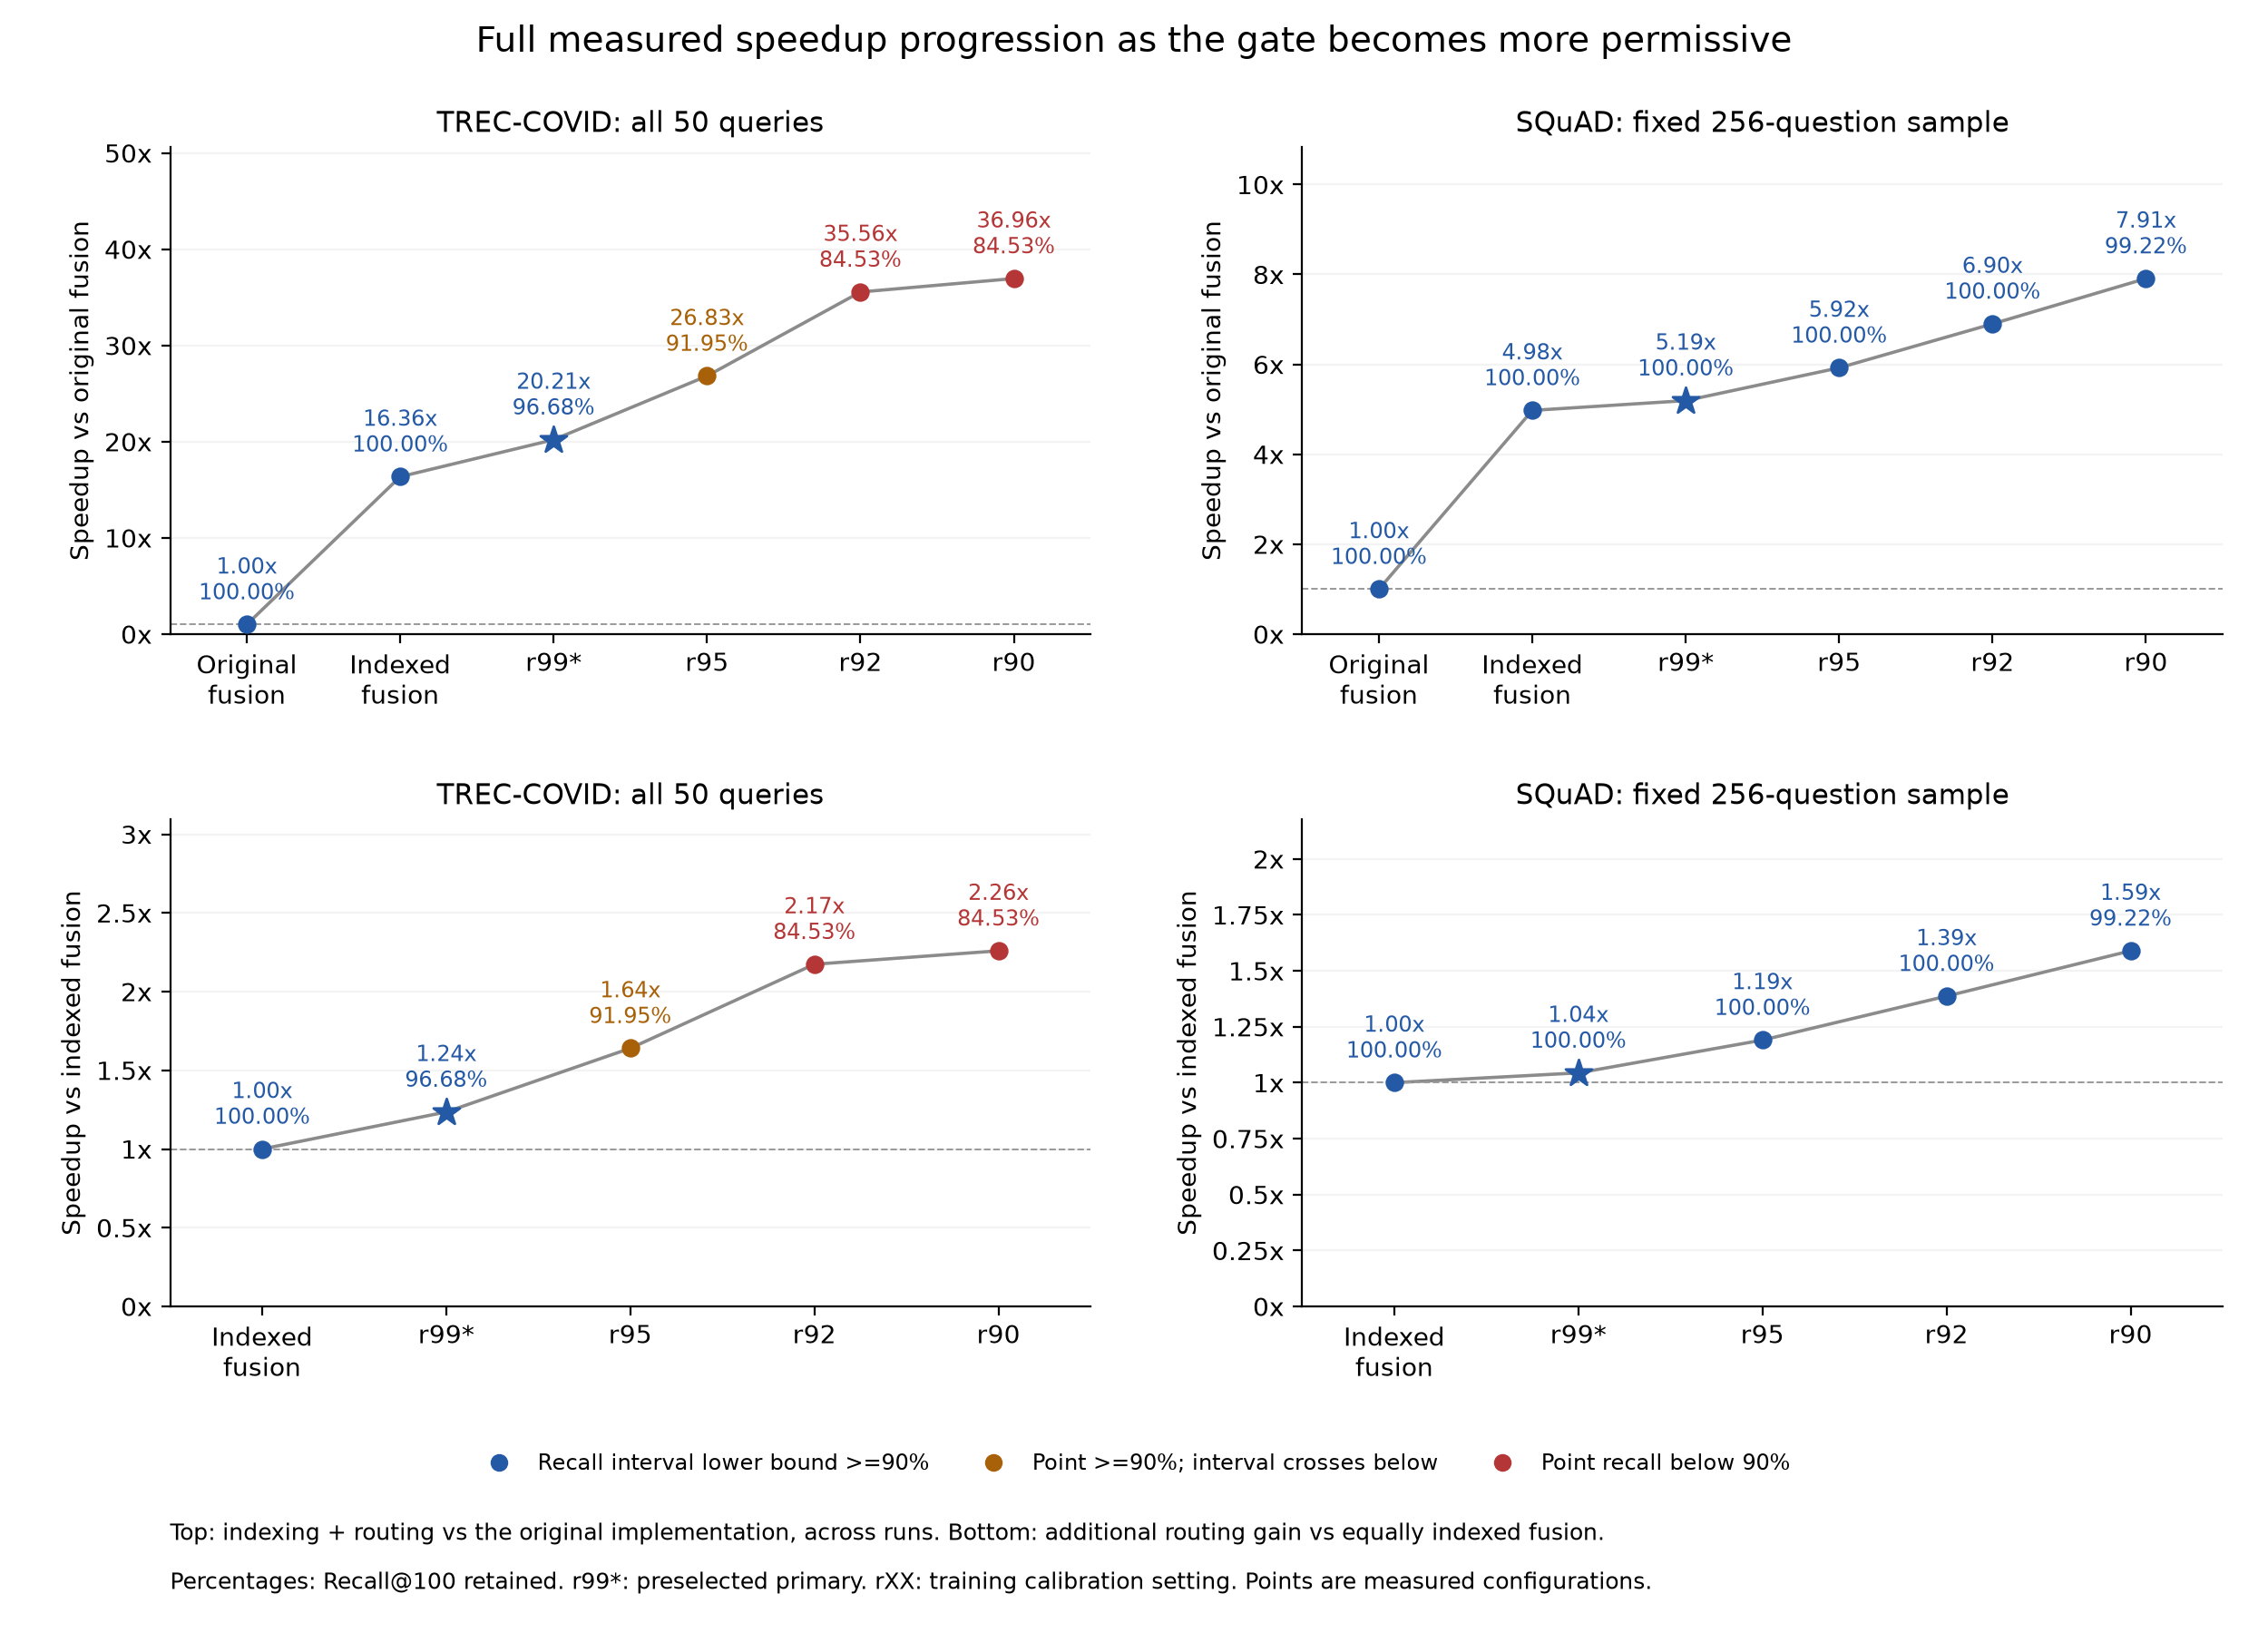
\includegraphics[width=\columnwidth]{figures/speedup_progression.png}
\caption{Measured speedup progression across cascade settings. The comparison with earlier fusion includes indexing and routing; the indexed-fusion comparison isolates the additional routing gain.}
\label{fig:speedup}
\end{figure}

\section{Experimental Protocol}
We evaluate the BEIR TREC-COVID collection with all 50 official queries and 171,332 documents \cite{beir}. The indexed SQuAD follow-up uses a predeclared SHA256-selected sample of 256 dev questions and the full 20,958-paragraph corpus \cite{squad}. Each SQuAD question is labeled relevant to its annotated source paragraph; other answer-bearing paragraphs may be unjudged. Full-query SQuAD retrieval was also run earlier, but the indexed sample is reported separately.

Additional transfer experiments used the NFCorpus development split (324 queries, 3,633 documents) and the SCIDOCS official test split (1,000 queries, 25,657 documents). Their original-backend measurements are kept separate from the indexed follow-ups. NFCorpus train supplies the gate's training labels; no evaluation qrels enter inference. The completed evaluation scope is summarized in Table~\ref{tab:scope}.

\begin{table*}[t]
\centering
\caption{Evaluation scope and timing coverage.}
\label{tab:scope}
\small
\begin{tabular}{lrrrrl}
\toprule
Study & Queries & Documents & Complete passes & Backend & Role in study\\
\midrule
NFCorpus development & 324 & 3,633 & 3 & Original & Development check (r92)\\
SCIDOCS test & 1,000 & 25,657 & 3 & Original & Frozen transfer check (r92)\\
TREC-COVID & 50 & 171,332 & 3 & Original & Paper-dataset extension (r90)\\
SQuAD dev & 10,570 & 20,958 & 1 & Original & Full-query retrieval result (r90)\\
TREC-COVID & 50 & 171,332 & 3 & Indexed & Engineering follow-up (r99 primary)\\
SQuAD dev sample & 256 & 20,958 & 3 & Indexed & Engineering follow-up (r99 primary)\\
\bottomrule
\end{tabular}
\end{table*}

The indexed SQuAD sample was selected by sorting query IDs by SHA256 of the dataset name, a null separator, and query ID, then taking the first 256. This fixed selection makes the sample reproducible and avoids choosing questions based on their benchmark outcomes. It does not make the sample equivalent to the full SQuAD query set.

The gate, weights, and thresholds were trained on NFCorpus train and frozen for evaluation. The indexed follow-ups use three warmed, randomized timing passes on a Tesla T4 with one CPU thread. Timings include query retrieval and routing, but exclude corpus encoding, index construction, model loading, downloads, and answer generation. The TREC follow-up uses all queries; the SQuAD follow-up uses only the declared sample. Results were independently rescored from raw relevance judgments. Query-paired bootstrap intervals use 1,000 resamples; they do not capture all hardware or session variation.

We kept development and confirmation decisions distinct. NFCorpus dev had already been inspected, and the 11-feature gate was calibrated on train. The r92 model, threshold, and confirmation protocol were fixed before SCIDOCS outcomes. NFCorpus test had been inspected earlier and was excluded from this calibration sequence. The indexed engineering follow-up selected the existing r99 policy as its primary against a 90\% floor before its indexed outcomes; some collection quality results, including TREC-COVID, were already known. We therefore describe this follow-up as an execution comparison on inspected data, not as an independent generalization test.

Recall retention is the ratio of mean Recall@100 for a method to mean Recall@100 for static fusion. It is not list overlap or a per-query guarantee and can exceed 100\%. We also report nDCG@10, MAP@10, and mean latency. We use two timing references: indexed fusion to measure the extra routing gain, and the earlier non-indexed fusion to show the combined indexing-plus-routing change across separate runs.

For query $q$ with judged relevant set $G_q$ and retrieved top-$K$ set $D_q^K$, recall is $|G_q\cap D_q^K|/|G_q|$. We average per-query recall before calculating retention. Thus, a retention of 96.68\% means that the method's mean recall equals 0.9668 times fusion's mean recall; it does not say that 96.68\% of relevant documents were retrieved. nDCG@10 measures graded ranking gain near the top, while MAP@10 summarizes precision at relevant ranks in the top 10. Neither metric is generated-answer accuracy.

Timing runs randomize query and method order and include warmups. GPU operations are synchronized around timed work. Each indexed run uses one Tesla T4 session and one CPU thread. We report the average of query latency observations across the three passes. Bootstrap intervals resample queries in paired form; timing intervals therefore reflect query variation in this session, not all hardware, software, or load variation. We do not include corpus encoding, neural model loading, data download, index construction, or LLM generation in the per-query latency.

\section{Results}
\subsection{Indexed TREC-COVID}
Table~\ref{tab:trec} reports all indexed TREC-COVID methods. The preselected r99 cascade reduced mean latency from 91.28 to 73.90 ms, a 19.04\% saving or 1.24$\times$ speedup relative to equally indexed fusion, while retaining 96.68\% of fusion Recall@100. Its query-bootstrap 95\% intervals were 93.58\%--98.75\% for recall retention and 9.47\%--30.11\% for time saved. The policy met the study's 90\% floor in this measured setting but missed its nominal 99\% target.

The secondary r95 point was faster, but its recall interval crossed below 90\%. SPLADE alone had higher observed recall and nDCG than the primary cascade at a lower mean latency; the cascade had higher MAP@10. Therefore, the cascade improved on fusion but was not the strongest measured choice under a recall-and-time objective.

\begin{table*}[t]
\centering
\caption{Indexed TREC-COVID: all 50 queries and the full corpus.}
\label{tab:trec}
\small
\begin{tabular}{lrrrrr}
\toprule
Method & Recall retained & nDCG@10 & MAP@10 & Mean ms & Speedup vs. fusion\\
\midrule
Static fusion & 100.00\% & 0.76323 & 0.01861 & 91.28 & 1.00$\times$\\
BM25 & 71.38\% & 0.54969 & 0.01145 & 8.11 & 11.25$\times$\\
Dense & 69.81\% & 0.47254 & 0.01054 & 30.41 & 3.00$\times$\\
SPLADE & 104.69\% & 0.72899 & 0.01662 & 52.77 & 1.73$\times$\\
r99 (primary) & 96.68\% & 0.72281 & 0.01769 & 73.90 & 1.24$\times$\\
r95 & 91.95\% & 0.70561 & 0.01742 & 55.66 & 1.64$\times$\\
r92 & 84.53\% & 0.65315 & 0.01499 & 41.99 & 2.17$\times$\\
r90 & 84.53\% & 0.65115 & 0.01499 & 40.41 & 2.26$\times$\\
\bottomrule
\end{tabular}
\end{table*}

Indexing alone changed fusion latency from 1493.23 ms to 91.28 ms, an observed 16.36$\times$ cross-run ratio. The primary cascade was 20.21$\times$ faster than earlier fusion across separate runs, but this combines indexing and routing. The additional cascade gain is 1.24$\times$ against indexed fusion.

\subsection{Indexed SQuAD sample}
On the fixed 256-question sample, r90 was 1.59$\times$ faster than indexed fusion and retained 99.22\% of its recall. The preselected r99 policy retained 100\% and was 1.04$\times$ faster. BM25 alone retained 95.70\% and averaged 1.03 ms, so it was the fastest listed method above a 90\% recall floor for this sample. These results do not represent all 10,570 SQuAD dev questions.

\begin{table*}[t]
\centering
\caption{Indexed SQuAD on the fixed 256-question sample.}
\label{tab:squad}
\small
\begin{tabular}{lrrrrr}
\toprule
Method & Recall retained & nDCG@10 & MAP@10 & Mean ms & Speedup\\
\midrule
Static fusion & 100.00\% & 0.80931 & 0.77059 & 29.55 & 1.00$\times$\\
BM25 & 95.70\% & 0.77869 & 0.75038 & 1.03 & 28.59$\times$\\
Dense & 95.70\% & 0.68778 & 0.63040 & 10.82 & 2.73$\times$\\
SPLADE & 98.83\% & 0.85440 & 0.82831 & 16.96 & 1.74$\times$\\
r99 (primary) & 100.00\% & 0.81020 & 0.77082 & 28.31 & 1.04$\times$\\
r95 & 100.00\% & 0.80277 & 0.76464 & 24.82 & 1.19$\times$\\
r92 & 100.00\% & 0.80287 & 0.76757 & 21.31 & 1.39$\times$\\
r90 & 99.22\% & 0.80092 & 0.76757 & 18.59 & 1.59$\times$\\
\bottomrule
\end{tabular}
\end{table*}

The r99 primary saved 4.19\% of mean time, with a query-bootstrap interval of 1.90\%--7.04\%. It exited on 14 of the 256 questions and retained every observed parent paragraph. The r90 setting exited on 39.84\% of queries, saved 37.08\% of mean time, and retained 99.22\%. Its recall-retention interval was 98.05\%--100\%, while its time-saving interval was 31.58\%--42.69\%. Despite this stronger sampled trade-off, r90 remains a secondary setting because r99 was preselected as the primary policy for the indexed follow-up.

The rank metrics give a different view from recall. SPLADE had the highest observed nDCG@10 and MAP@10 in this sample. BM25, though much faster, retained 95.70\% of fusion's Recall@100 and achieved nDCG@10 of 0.77869. The sample's perfect recall retention for r92, r95, and r99 is an observed property of these questions; it does not imply zero loss on the remaining SQuAD queries.

\subsection{Earlier backend and transfer results}
The indexed follow-ups came after initial experiments with the original scorer. Table~\ref{tab:transfer} shows the primary policy reported in each earlier study. These runs answer a separate question from the indexed comparisons: how did the frozen gate transfer before BM25 indexing reduced the first-stage cost?

\begin{table*}[t]
\centering
\caption{Primary results from the original-backend evaluations.}
\label{tab:transfer}
\small
\begin{tabular}{lrrrrr}
\toprule
Collection & Policy & Recall retained & Fusion ms & Cascade ms & Time saved\\
\midrule
NFCorpus dev & r92 & 94.74\% & 23.61 & 18.18 & 23.00\%\\
SCIDOCS test & r92 & 90.01\% & 159.51 & 150.69 & 5.53\%\\
TREC-COVID & r90 & 84.53\% & 1493.23 & 1440.00 & 3.56\%\\
SQuAD dev, all queries & r90 & 99.38\% & 148.26 & 139.19 & 6.12\%\\
\bottomrule
\end{tabular}
\end{table*}

The transfer results show that training retention targets did not consistently transfer. Every nominal setting missed its target on SCIDOCS and TREC-COVID, while the selected SQuAD r90 result retained 99.38\%. On SCIDOCS, the r92 estimate was 90.01\%, but its 95\% recall interval ranged from 88.27\% to 91.61\%, crossing the 90\% floor. The original TREC r90 result retained 84.53\% and saved only 3.56\% mean time. That weak time result is consistent with BM25 consuming most of the end-to-end latency.

Standalone retrievers also set a demanding baseline. Dense retrieval retained 99.77\% of fusion recall at 6.62 ms on NFCorpus dev. On SCIDOCS, Dense retained 109.65\%, took 10.14 ms, and led BM25, SPLADE, and fusion on the reported quality metrics. These findings motivated the explicit standalone comparisons in the paper-dataset follow-ups.

\begin{figure}[t]
\centering
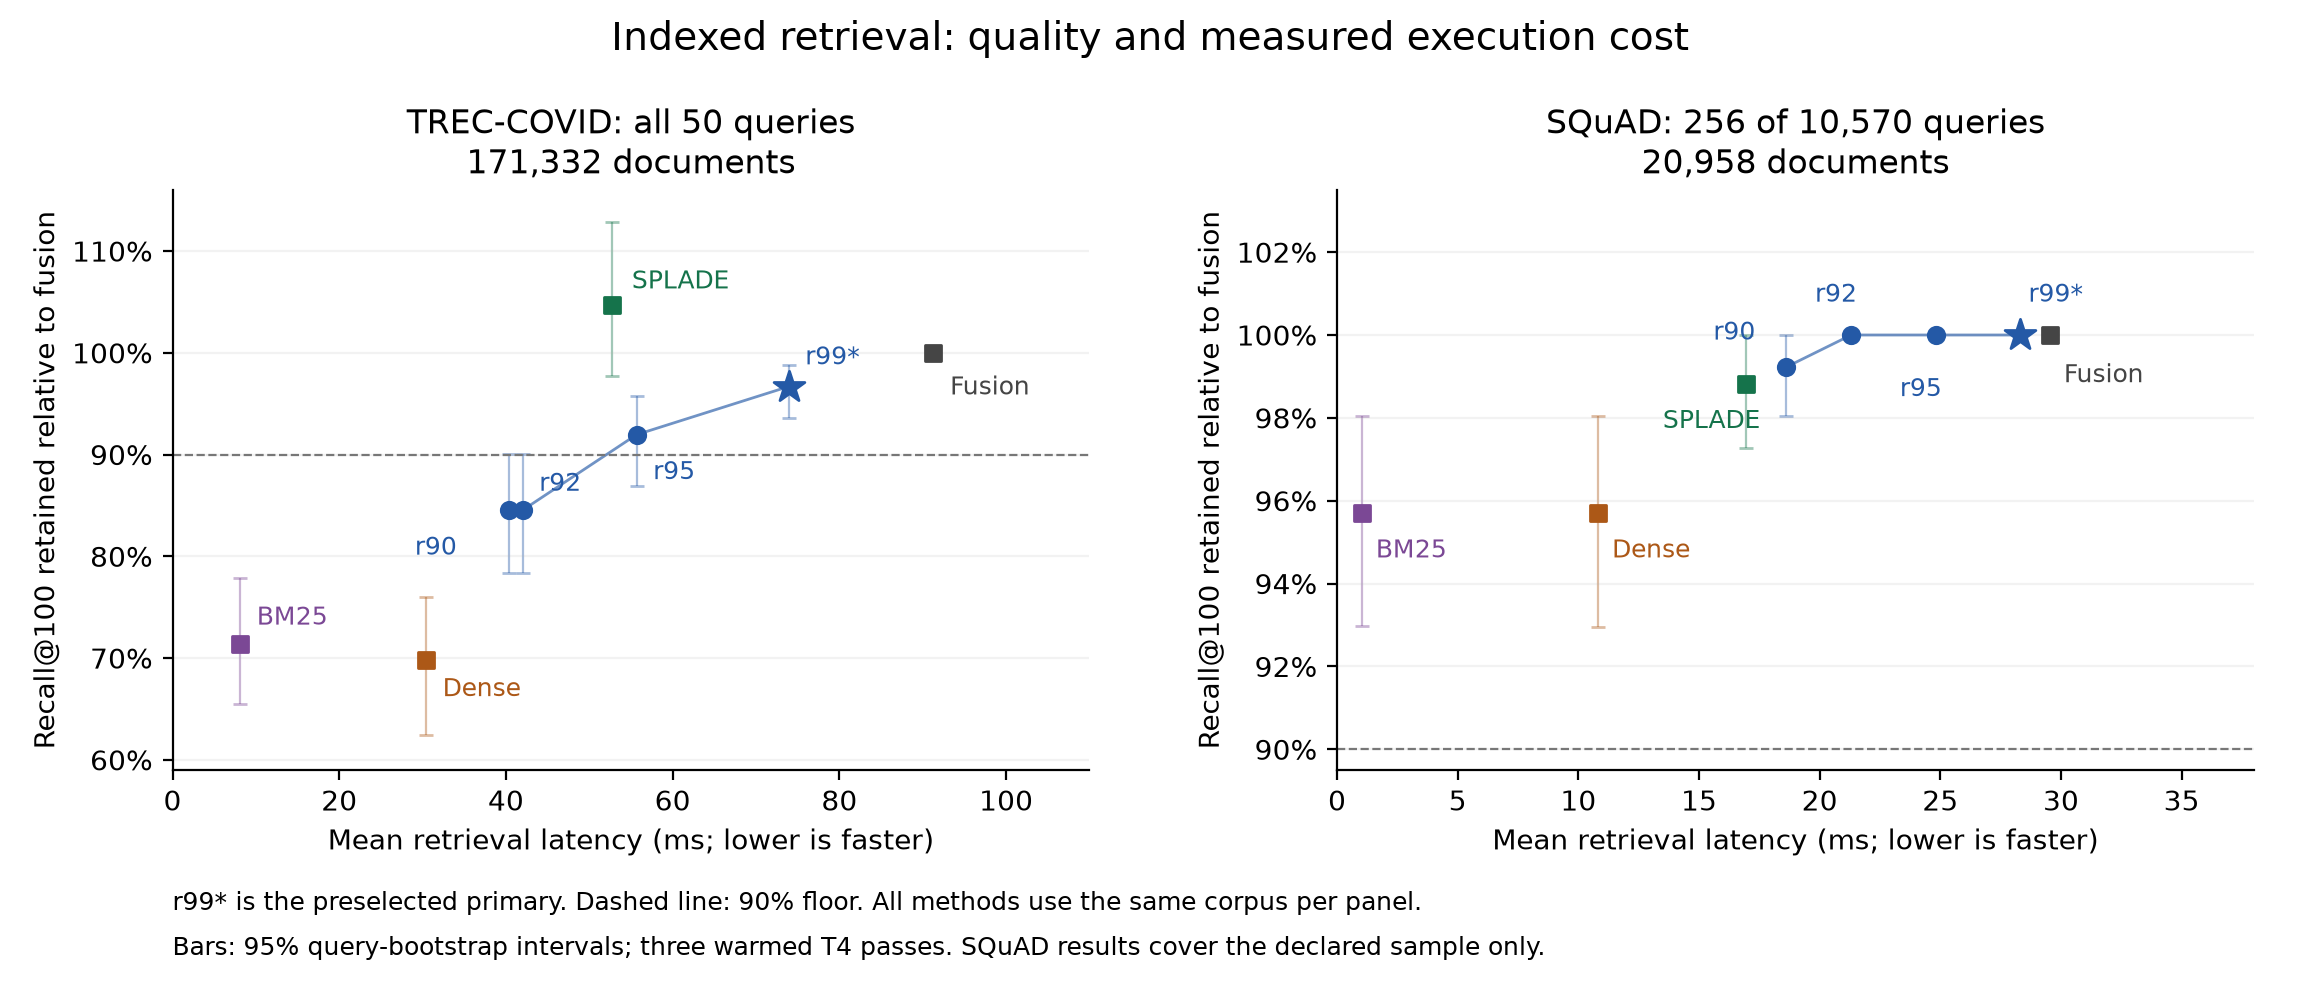
\includegraphics[width=\columnwidth]{figures/indexed_quality_latency.png}
\caption{Recall retention and mean latency for indexed methods. SQuAD results use the declared 256-question sample.}
\label{fig:quality-latency}
\end{figure}

\section{Discussion}
The first-stage cost determined whether routing could save time. On the original TREC implementation, BM25 took 1410.14 ms of the 1493.23 ms full-fusion latency. After indexing, BM25 averaged 8.11 ms, allowing skipped neural inference to reduce the cascade's mean time against indexed fusion. This component comparison is an observed 173.78$\times$ BM25 scoring ratio across separate runs; it is not the cascade's end-to-end speedup. Dense latency stayed close to 30 ms and SPLADE near 53 ms in the indexed TREC run, so the BM25 change removed work from the lexical branch rather than making the neural models faster.

Calibration did not guarantee transfer. All nominal settings missed their targets on TREC-COVID in the original-backend experiment, and the indexed TREC r99 policy also fell short of 99\%. The indexed SQuAD sample showed no recall loss for r92, r95, and r99, but this is an observation on 256 questions, not a guarantee for unmeasured queries.

Standalone results matter. SPLADE was a better recall/time choice than the primary cascade on TREC-COVID, while BM25 alone exceeded a 90\% retention floor at far lower time on the indexed SQuAD sample. A cascade can beat static fusion and still be unnecessary when one retriever already meets the target.

The evaluation has limits. It uses one GPU type and one timing session per indexed follow-up; p95 improvement was not established. Index construction, memory, updates, production concurrency, energy, and generated-answer quality were outside the measurement. Full NQ, HotpotQA, CoQA, and direct testing on Elasticsearch/ELSER remain future work. The indexed TREC follow-up used already-inspected quality results, so it tests execution on known data rather than independent quality generalization.

The SQuAD setup also has a label limitation. Each dev question is judged relevant to its annotated source paragraph, even though another paragraph in the corpus might contain a valid answer. This is a retrieval benchmark under the available labels, not a complete assessment of every answer-bearing passage. TREC-COVID has only 50 topics, so query-level intervals remain sensitive to individual topics. The bootstrap intervals quantify resampling variability across the evaluated queries; they cannot establish results on other hardware or on a new collection.

Finally, a quality floor does not uniquely define the best system. If the objective is only to exceed 90\% retention on the indexed SQuAD sample, BM25 alone is faster than every cascade. On TREC-COVID, SPLADE alone has better recall and nDCG than the primary cascade, although the cascade has higher MAP@10. A practical system would need its application to specify which quality measures matter and then compare all methods under that requirement. We do not select a new objective after observing the results.

\section{Conclusion}
We implemented a BM25-first cascade and a compatible postings-based BM25 scorer, then measured the cascade against equally indexed fusion and standalone retrievers. The primary indexed TREC-COVID cascade saved 19.04\% mean time while retaining 96.68\% of fusion Recall@100; on the fixed SQuAD sample, the fastest cascade saved 37.08\% while retaining 99.22\%. Indexing accounts for a substantial part of the larger comparisons against the earlier implementation. The results support a measured execution trade-off within our Python setup, while standalone baselines and dataset scope prevent a claim of overall superiority or acceleration of the original Blended RAG system.

\begin{thebibliography}{00}
\bibitem{blended} K. Sawarkar, A. Mangal, and S. R. Solanki, ``Blended RAG: Improving RAG (Retriever-Augmented Generation) Accuracy with Semantic Search and Hybrid Query-Based Retrievers,'' arXiv:2404.07220, 2024.
\bibitem{adaptive} N. Arabzadeh, X. Yan, and C. L. A. Clarke, ``Predicting Efficiency/Effectiveness Trade-offs for Dense vs. Sparse Retrieval Strategy Selection,'' arXiv:2109.10739, 2021.
\bibitem{bm25s} X. H. Lu, ``BM25S: Orders of Magnitude Faster Lexical Search via Eager Sparse Scoring,'' arXiv:2407.03618, 2024.
\bibitem{beir} N. Thakur et al., ``BEIR: A Heterogeneous Benchmark for Zero-shot Evaluation of Information Retrieval Models,'' in \emph{NeurIPS Datasets and Benchmarks}, 2021.
\bibitem{squad} P. Rajpurkar, J. Zhang, K. Lopyrev, and P. Liang, ``SQuAD: 100,000+ Questions for Machine Comprehension of Text,'' in \emph{Proc. EMNLP}, 2016.
\bibitem{splade} T. Formal, B. Piwowarski, and S. Clinchant, ``SPLADE: Sparse Lexical and Expansion Model for First Stage Ranking,'' in \emph{Proc. SIGIR}, 2021.
\bibitem{sbert} N. Reimers and I. Gurevych, ``Sentence-BERT: Sentence Embeddings using Siamese BERT-Networks,'' in \emph{Proc. EMNLP-IJCNLP}, 2019.
\end{thebibliography}
\end{document}
